\section{Macroelement Spaces}

%%%%%%%%%%%%%%%%%%%%%%%%%%%%%%%%%%%%%%%%%%%%%%%%%%%%%%%%%%%%%%%%%%%%%
\royslide{$C^1$ Finite Element Spaces}{
In Galerkin formulations of plate bending, streamfunction viscous
flow, Cahn-Hilliard interfaces, and surface
tension driven films, we find integrated products
of second derivatives of the solution and test functions.

With variational problems posed on subspaces of $H^2(\Omega)$,
conforming finite element approximations
require $H^2$ conforming functions.

A $C^1$ continuous (and $W^{2,\inf}$ bounded, $W^{2,p}$ conforming)
finite element is needed, e.g.:

\royitemizebegin
	\item Powell-Sabin 6-split triangle
	\item Powell-Sabin-Heindl (PSH) 12-split triangle
	\item Hsieh-Clough-Tocher (HCT) 3-split triangle
\royitemizeend
}



%%%%%%%%%%%%%%%%%%%%%%%%%%%%%%%%%%%%%%%%%%%%%%%%%%%%%%%%%%%%%%%%%%%%%
\royslide{Macroelements}{

Constraining polynomial triangles to $C^1$ continuity
requires quintic polynomials.  To use lower $p$,
we construct macroelements by
subdividing each triangle, using piecewise polynomial functions
with continuity constraints along interior edges.

\begin{center}
\fbox{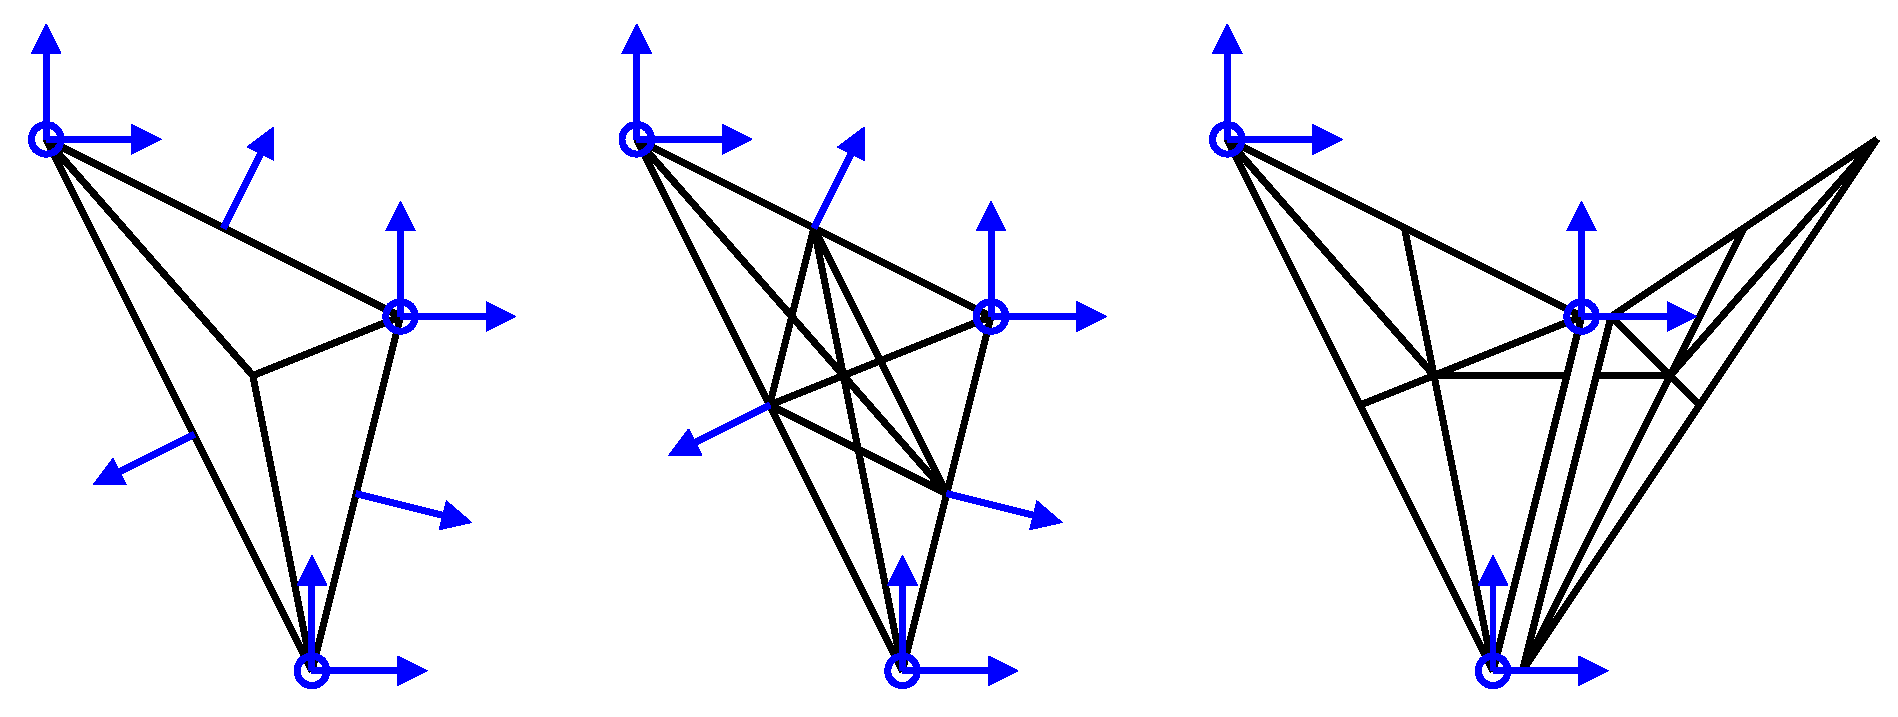
\includegraphics[width=.9\textwidth]{figs/triangles}}
\end{center}

% Mention additional ``raw'' degrees of freedom

% Mention spectral methods

}



%%%%%%%%%%%%%%%%%%%%%%%%%%%%%%%%%%%%%%%%%%%%%%%%%%%%%%%%%%%%%%%%%%%%%
%\royslide{Constructing Macroelements}{
%
%To reliably construct a macroelement basis:
%
%\begin{itemize}
%\item Number the ``raw'' degrees of freedom
%\item ``Write'' all constraints as matrix rows
%\item Put constraint matrix in row reduced form
%\item Add boundary DoF equations (checking each for
%linear independence)
%\item If necessary, make matrix square with interior DOF
%equations (again checking for linear independence)
%\item Invert matrix, multiply by $\hat{e}_i$ to get basis coefficients
%corresponding to the DOF on row $i$
%\end{itemize}
%
%}


%%%%%%%%%%%%%%%%%%%%%%%%%%%%%%%%%%%%%%%%%%%%%%%%%%%%%%%%%%%%%%%%%%%%%
%\royslide{Powell-Sabin 6-split}{
%\begin{center}
%\fbox{\includegraphics[width=.7\textwidth]{figs/Basis_psrt}}
%\end{center}
%}


%\royslide{Powell-Sabin-Heindl 12-split}{
%\begin{center}
%\fbox{\includegraphics[width=.7\textwidth]{figs/Basis_hrt}}
%\end{center}
%}


%\royslide{Clough-Tocher 3-split}{
%\begin{center}
%\fbox{\includegraphics[width=.7\textwidth]{figs/Basis_ctrt}}
%\end{center}
%}


%%%%%%%%%%%%%%%%%%%%%%%%%%%%%%%%%%%%%%%%%%%%%%%%%%%%%%%%%%%%%%%%%%%%%
\royslide{Approximation Convergence}{
PSH and HCT triangles exactly
reproduce quadratics and cubics $(k \equiv 2, 3)$,
respectively.  Standard interpolation, $H^2$ approximation rules
apply for $w \in H^n(\Omega) \subset H^{k+1}(\Omega)$, but $L_2$
approximation on PSH triangles is suboptimal.

\begin{eqnarray*}
%P_h(f) & \equiv & \sum_{i=1}^{N} \sigma_i(f)\phi_i \\
\norm{w - P_h w}_{H^m(\Omega)}
& \leq & C h^{n-m} \abs{w}_{H^n(\Omega)} \\
%\norm{u - u_h}_{H^2(\Omega)} & \leq & \left( 1 + \frac{\norm{B}}{\alpha_h} \right)
\norm{u - u_h}_{H^2(\Omega)} & \leq & 
C h^{n-2} \norm{u}_{H^n(\Omega)} \\
\norm{u - u_h}_{H^r(\Omega)} & \leq & 
C h^{\min \left(2(k+1-m),k+1-r,n-r\right)} \norm{u}_{H^n(\Omega)}
\end{eqnarray*}
}


%%%%%%%%%%%%%%%%%%%%%%%%%%%%%%%%%%%%%%%%%%%%%%%%%%%%%%%%%%%%%%%%%%%%%
%\royslide{$H^2$ Approximation Convergence}{
%
%Given that our operator is bounded and satisfies an inf-sup
%condition on our $H^2$ conforming function space $P$, Galerkin
%orthogonality (the C\'{e}a lemma) gives us the expected (linear for
%Powell-Sabin, quadratic for Clough-Tocher) asymptotic error in the
%$H^2$ norm, for problems with sufficiently smooth (contained in
%$H^n(\Omega)$, for $n \equiv k + 1$) solutions:
%
%\vspace{-2em}
%\begin{eqnarray*}
%\alpha_h & \equiv & \inf_{v_h \in P} \sup_{w_h \in P}
%\frac{B(v_h,w_h)}{\norm{v_h}_P \norm{w_h}_P} \\
%\norm{u - u_h}_{H^2(\Omega)} & \leq & \left( 1 + \frac{\norm{B}}{\alpha_h} \right)
%\inf_{v_h \in P} \norm{u - v_h}_{H^2(\Omega)} \\
%& \leq & \left( 1 + \frac{\norm{B}}{\alpha_h} \right)
%\norm{u - P_h u}_{H^2(\Omega)} \\
%& \leq & \left( 1 + \frac{\norm{B}}{\alpha_h} \right)
%C h^{n-2} \abs{u}_{H^n(\Omega)} \\
%\end{eqnarray*}
%\vspace{-2em}
%
%}


%%%%%%%%%%%%%%%%%%%%%%%%%%%%%%%%%%%%%%%%%%%%%%%%%%%%%%%%%%%%%%%%%%%%%
%\royslide{$L_2$ Approximation Convergence}{
%
%HCT elements obtain an additional power of $h$ in $H^2$
%convergence.
%The difference grows in the $L_2$
%norm.  Defining $\eta \equiv \min \left(2(k+1-m),k+1-r,n-r\right)$,
%if $u_h$ is the Galerkin approximation to a bilinear problem on
%$H^m(\Omega)$,
%
%\begin{eqnarray*}
%\norm{u - u_h}_{H^r(\Omega)} \leq C h^{\eta} \norm{u}_{H^n(\Omega)}
%\end{eqnarray*}
%
%For $k = 3$, or $k = 2, r \geq 1$, this is the standard rule
%of thumb.
%
%For fourth order problems ($m = 2$), quadratic elements ($k = 2$), and
%the $L_2$ norm ($r = 0$), the $\eta \leq 2(k+1-m)$ term dominates.
%}
